\lab{K-Means Clustering}{K-Means Clustering}
\objective{Understand the basics of \emph{k-means} clustering, and apply to the problem of clustering earthquake epicenters.}

\subsection*{Clustering}
In Lab \ref{lab:pca}, we analyzed the iris dataset using PCA; we have reproduced the first two principal components of the iris data in Figure \ref{fig:iris_data}.
Upon inspection, a human can easily see that there are two very distinct groups of irises.
Can we create an algorithm to identify these groups without human supervision?
This task is called \emph{clustering}, an instance of \emph{unsupervised learning}.

\begin{figure}
\centering
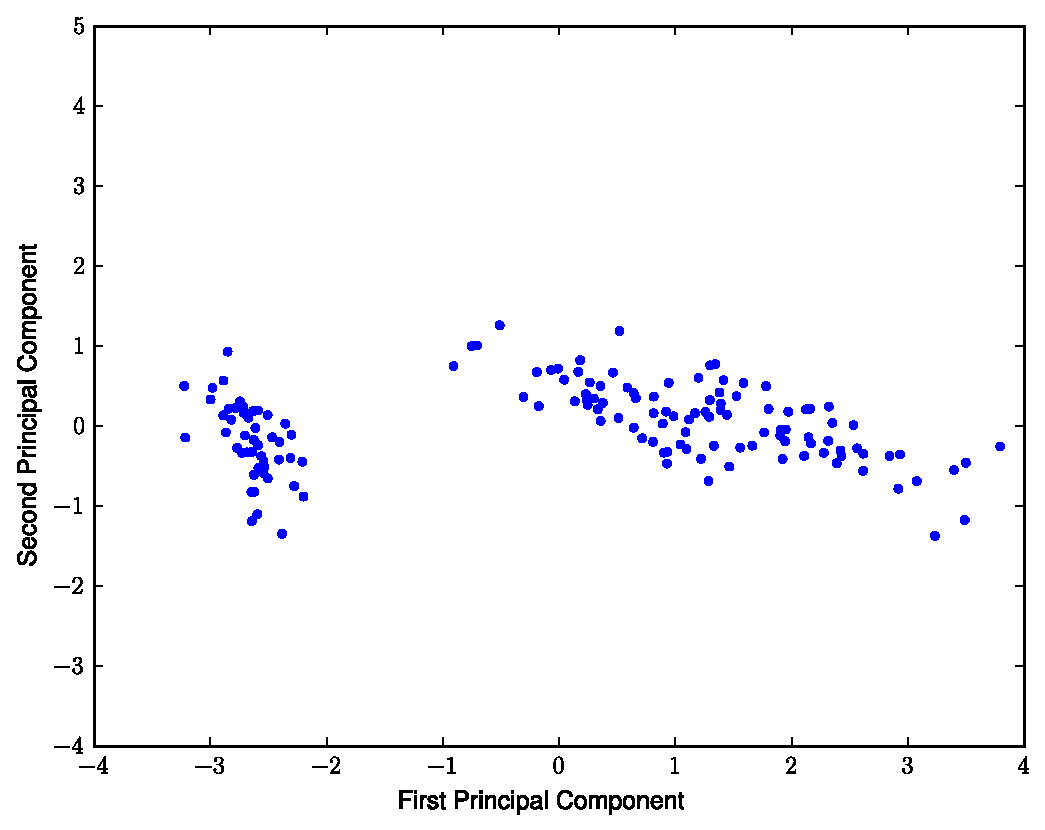
\includegraphics[width=\textwidth]{iris_pca.pdf}
\caption{The first two principal components of the iris dataset.}
\label{fig:iris_data}
\end{figure}

The objective of clustering is to find a partition of the data such that points in the same subset will be ``close'' according to some metric.
The metric used will likely depend on the data, but some obvious choices include Euclidean distance and angular distance.
Throughout this lab we will use the metric $d(x,y) = \|x-y\|_2$, the Euclidean distance between $x$ and $y$.

More formally, suppose we have a collection of $\mathbb{R}^K$-valued observations $X = \{x_1,x_2,\ldots,x_n\}$.
Let $N \in \mathbb{N}$ and let $\mathcal{S}$ be the set of all $N$-partitions of $X$, where an $N$-partition is a partition with exactly $N$ nonempty elements.
We can represent a typical partition in $\mathcal{S}$ as $S = \{S_1,S_2,\ldots,S_N\}$, where
\[
X = \bigcup_{i=1}^N S_i
\]
and
\[
|S_i| > 0, \qquad i=1,2,\ldots,N.
\]
We seek the $N$-partition $S^*$ that minimizes the within-cluster sum of squares, i.e.
\[
S^* = \underset{S\in\mathcal{S}}{\arg\min} \sum_{i=1}^N\sum_{x_j\in S_i}\|x_j-\mu_i\|_2^2,
\]
where $\mu_i$ is the mean of the elements in $S_i$, i.e.
\[
\mu_i = \frac{1}{|S_i|}\sum_{x_j\in S_i}x_j.
\]

\subsection*{The \emph{K-Means} Method}
Finding the global minimizing partition $S^*$ is generally intractable since the set of partitions can be very large indeed,
but the \emph{k-means} algorithm is a heuristic approach that can often provide reasonably accurate results.


We begin by specifying an initial cluster mean $\mu_i^{(1)}$ for each $i = 1, \cdots, N$ (this can be done by random initialization, or according to some heuristic).
For each iteration, we adopt the following procedure.
Given a current set of cluster means $\mu^{(t)}$, we find a partition $S^{(t)}$ of the observations such that
\begin{equation*}
S_{i}^{(t)} = \{x_j \; : \; \|x_j - \mu_{i}^{(t)}\|_2^2 \leq \|x_j - \mu_{l}^{(t)}\|_2^2,\,\,\,  l = 1, \cdots, N\}.
\end{equation*}
We then update our cluster means by computing for each $i = 1, \cdots, N$.
We continue to iterate in this manner until the partition ceases to change.



Examine Figure \ref{fig:iris_clusterings}, which shows two different clusterings of the iris data produced by the \emph{k-means} algorithm.
Note that the quality of the clustering can depend heavily on the initial cluster means.
We can use the within-cluster sum of squares as a measure of the quality of a clustering (a lower sum of squares is better).
Where possible, it is advisable to run the clustering algorithm several times, each with a different initialization of the means,
and keep the best clustering.
Note also that it is possible to have very slow convergence.
Thus, when implementing the algorithm, it is a good idea to terminate after some specified maximum number of iterations.

\begin{figure}[h]
	\centering
	\begin{tabular}{cc}
	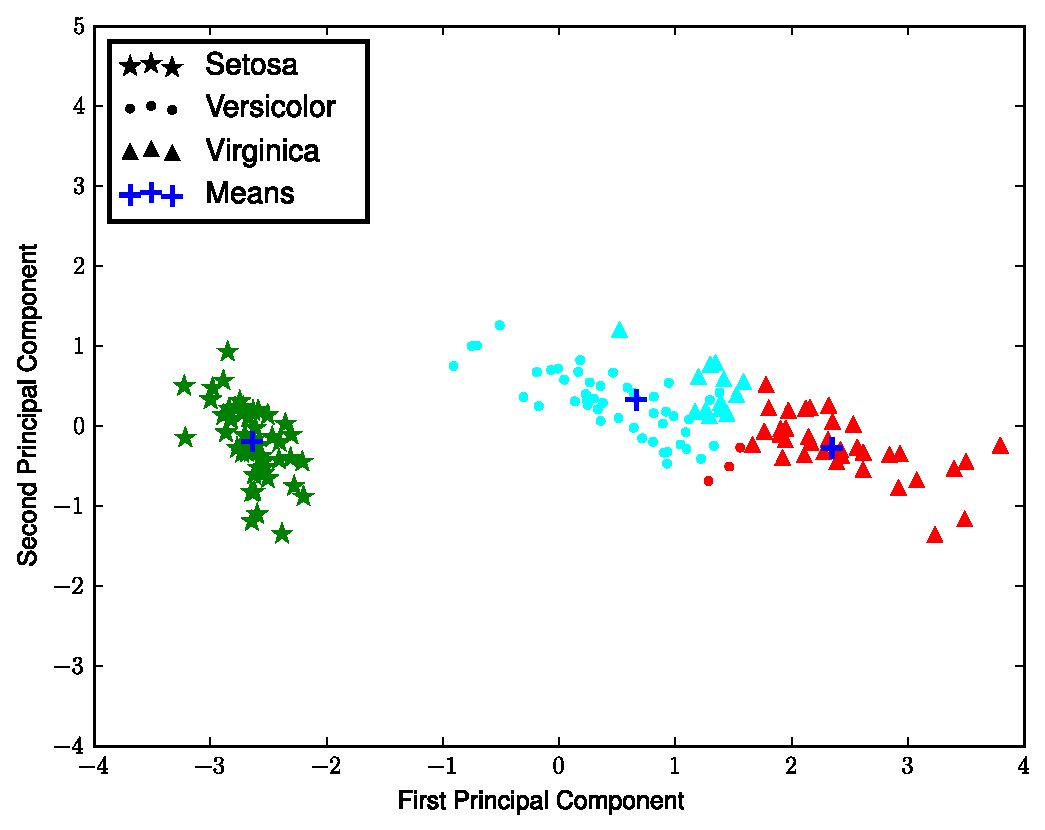
\includegraphics[width=.49\textwidth]{iris_means_1.pdf} &
	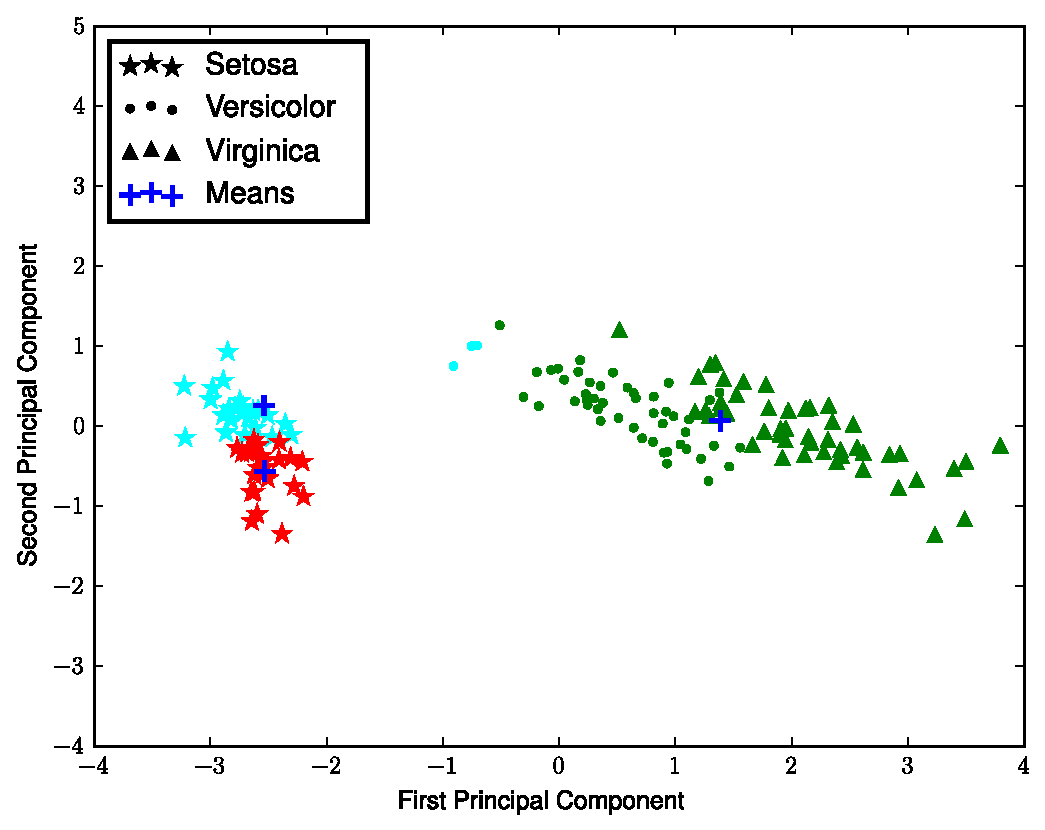
\includegraphics[width=.49\textwidth]{iris_means_2.pdf}
	\end{tabular}
	\caption{Two different K-Means clusterings for the iris dataset.
            Notice that the clustering on the left predicts the flower species to a high degree of accuracy,
            while the clustering on the right is less effective.}
    \label{fig:iris_clusterings}
\end{figure}

\begin{problem}
Implement the \emph{k-means} algorithm using the following function declaration.

\begin{lstlisting}
def kmeans(data,n_clusters,init='random',max_iter=300):
    """
    Cluster a dataset using the k-means algorithm.

    Parameters
    ----------
    data : ndarray of shape (n,k)
        Each row is an observation.
    n_clusters : int
        The number of clusters.
    init : string or ndarray of shape (n_clusters,k)
        If init is the string 'random', then randomly initialize the cluster means.
        Else, the initial cluster means are given by the rows of init.
    max_iter : int
        The maximum allowable number of iterations.

    Returns
    -------
    means : ndarray of shape (n_cluster,k)
        The final cluster means, given as the rows.
    labels : ndarray of shape (n,)
        The i-th entry is an integer in [0,n_clusters-1] indicating
        which cluster the i-th row of data belongs to relative to
        the rows of means.
    measure : float
        The within-cluster sum of squares quality measure.
    """
    pass
\end{lstlisting}

Test your function on the first two principal components of the iris dataset.
Run it 10 times, using a different random initialization of the means each time.
Retain the clustering with the smallest within-cluster sum of squares.
Your clustering should be similar to the first clustering in Figure \ref{fig:iris_clusterings}.
\end{problem}

\subsection*{Detecting Active Earthquake Regions}
Suppose we are interested in learning about which regions are prone to experience frequent earthquake activity.
We could make a map of all earthquakes over a given period of time and examine it ourselves, but this, as an unsupervised learning problem, can be solved using our k-means clustering tool.

Our data is contained in 6 text files, each with earthquake data throughout the world covering a time period of one month, giving us data from January 2010 through June 2010.
These files contain a lot of information which isn't of interest to us at the present time; all we would like to extract from them is the location of each earthquake, which appears in characters $21$ through $33$ of each line.
Characters $21$ through $26$ contain the latitude of each epicenter, character $26$ denoting North or South, and characters $27$ through $33$ contain the longitude of each epicenter, character $33$ denoting East or West.
We need to divide each value by $1,000$ to represent these as degrees and decimals.
\begin{figure}
	\centering
	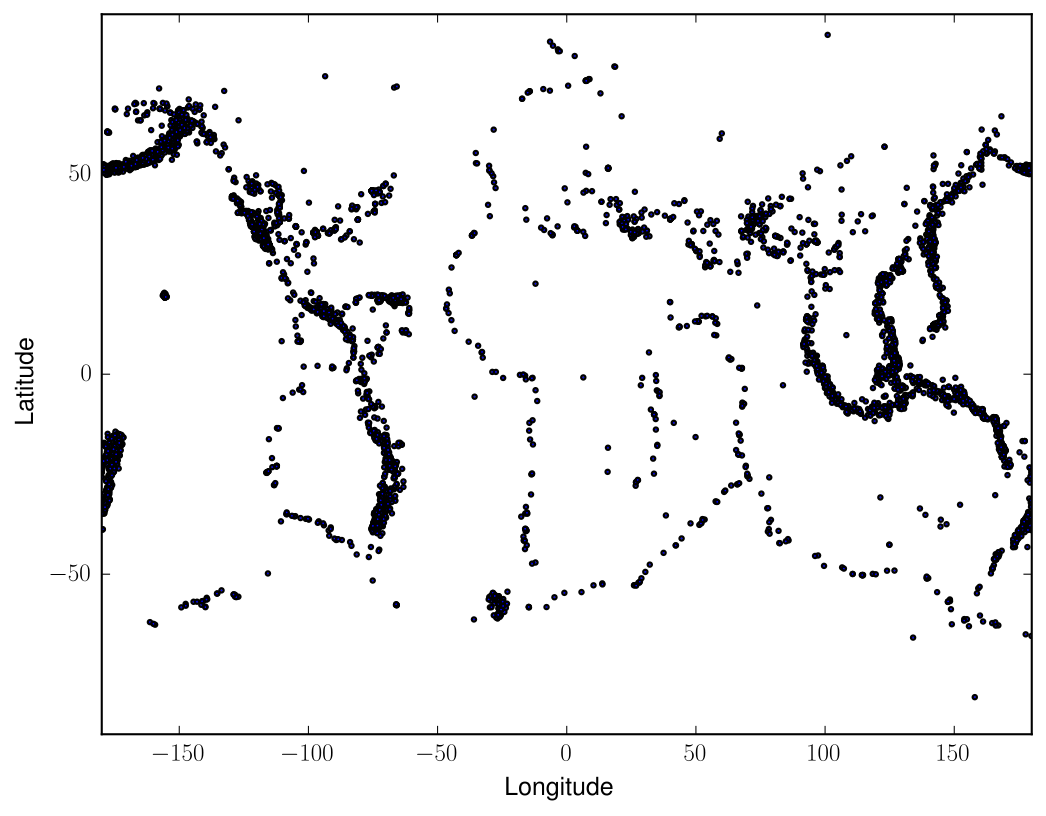
\includegraphics[width=\textwidth]{earthquakes.png}
	\caption{Earthquake epicenters over a 6 month period.}
	\label{fig:earthquakes}
\end{figure}
\begin{problem}
Load the earthquake data into a $n\times 2$ array, where each row gives the longitude and latitude of an earthquake in degrees.
Multiply South latitudes and West longitudes by $-1$.
Create a scatter plot of the resulting data. You should be able to see the outlines of some of the continents and tectonic plates (since these are often areas of significant seismic activity). Your plot should match Figure \ref{fig:earthquakes}.
\end{problem}

We want to cluster this data into active earthquake regions.
For this task, we might think that we can regard any epicenter as a point in $\mathbb{R}^{2}$ with coordinates being their latitude and longitude.
This, however, would be incorrect, because the earth is not flat. We must recognize that latitude and longitude are best viewed as a variation of spherical coordinates in $\mathbb{R}^{3}$, and we should interpret them as such.
Since our \emph{k-means} algorithm is based on Euclidean distance, we need to transform our data into 3-dimensional Euclidean coordinates.

A simple way to accomplish this transformation is to first transform the latitude and longitude values to spherical coordinates, and then to Euclidean coordinates.
Recall that a spherical coordinate in $\mathbb{R}^3$ is a triple $(r,\theta,\varphi)$, where $r$ is the distance from the origin, $\theta$ is the radial angle in the $xy$-plane from the $x$-axis,
and $\varphi$ is the angle from the $z$-axis. In our earthquake data, the longitude is already the appropriate $\theta$ value, and the $\varphi$ value (in degrees) is simply $90^\circ$ minus the latitude.
For simplicity, we can take $r=1$, since the earth is roughly a sphere.
We can then transform to Euclidean coordinates using the following relationships:
\begin{align*}
r & = \sqrt{x^{2} + y^{2} + z^{2}} & x & = r \sin \varphi \cos \theta \\
\varphi & = \arccos \frac{z}{r} & y & = r \sin \varphi \sin \theta \\
\theta & = \arctan \frac{y}{x} & z & = r \cos \varphi
\end{align*}

\begin{problem}
Transform your earthquake data into three dimensional Euclidean coordinates.
Be sure to consider if and when you need to transform your data from degrees to radians.
\end{problem}

We are now ready to cluster the earthquake data using the Euclidean coordinates.
We need to address one further issue, however.
Notice that each earthquake data point has norm 1 in Euclidean coordinates, since it lies on the surface of a sphere of radius 1.
We also need to ensure that our cluster means have norm 1.
Otherwise, the means can't be interpreted as locations on the surface of the earth.
Furthermore, the \emph{k-means} algorithm will struggle to find good clusters.
A solution to this problem is to normalize the mean vectors at each iteration, so that they are always unit vectors.
Thus, we need to add optional functionality to our \li{kmeans} function.
\begin{figure}
	\centering
	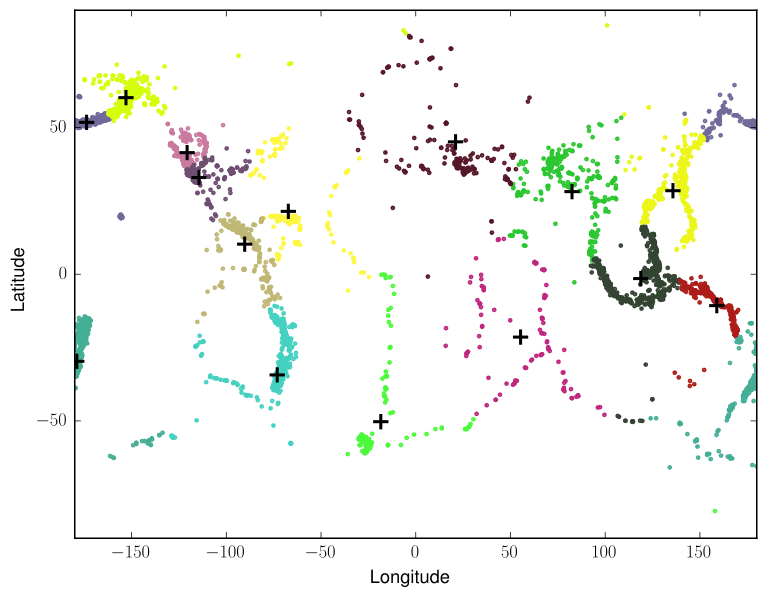
\includegraphics[width=\textwidth]{earthquake_clusters.png}
	\caption{Earthquake epicenter clusters with $N = 15$.}
	\label{fig:earthquakeclusters}
\end{figure}

\begin{problem}
Add a keyword argument \li{normalize=False} to your \li{kmeans} function, and add code to normalize the means at each iteration, should this argument be set to \li{True}.
Use your function to cluster the earthquake data into 15 clusters. Run this 10 times, keeping the best clustering.
Transform the cluster means back to latitude and longitude coordinates (when calculating $\theta$ using the inverse tangent, use \li{numpy.arctan2} or \li{math.arctan2},
so that that correct quadrant is chosen).
Create a scatter plot showing each cluster mean, along with the earthquake epicenters color-coded according to their cluster. Your plot should resemble that of Figure \ref{fig:earthquakeclusters}.
\end{problem}

Though plotting our results in two dimensions gives us a good picture, we can see that this is not entirely accurate.  There are points that appear to be closer to a different cluster center than the one to which they belong.  This comes from viewing the results in only two dimensions.  When viewing in three dimensions, we can see more clearly the accuracy of our results.  
\begin{problem}
Add a keyword argument \li{3d=False} to your \li{kmeans} function, and add code to show the three-dimensional plot instead of the two-dimensional scatter plot should this argument be set to \li{True}.  Maintain the same color-coding scheme as before.  Use \li{mpl_toolkits.mplot3d.Axes3D} to make your plot.
\end{problem}


\subsection*{Spectral Clustering}
We now turn to another method for solving a clustering problem, namely that of Spectral Clustering.  As you can see in Figure ???, it can cluster data not just by its location on a graph, but can even separate shapes that overlap others into distinct clusters.  It does so by utilizing the spectral properties of a Laplacian matrix.  Different types of Laplacian matrices can be used.  In order to construct a Laplacian matrix, we first need to create a graph of vertices and edges from our data points.  This graph can be represented as a symmetric matrix $W$ where $w_{ij}$ represents the edge from $x_i$ to $x_j$.  In the simplest approach, we can set $w_{ij} = 1$ if there exists an edge and $w_{ij} = 0$ otherwise.  However, we are interested in the similarity of points, so we will weight the edges by using a \emph{similarity measure}.  Points that are similar to one another are assigned a high similarity measure value, and dissimilar points a low value.  One possible measure is the \emph{Gaussian similarity function}, which defines the similarity between distinct points $x_i$ and $x_j$ as
\begin{equation*}
s(x_i,x_j) = e^{- \frac{\| x_i - x_j \| ^2}{2 \sigma ^2}}
\end{equation*}
for some set value $\sigma$.

Note that some similarity functions can yield extremely small values for dissimilar points.  We have several options for dealing with this possibility.  One is simply to set all values which are less than some $\epsilon$ to be zero, entirely erasing the edge between these two points.  Another option is to keep only the $T$ largest-valued edges for each vertex.  Whichever method we choose to use, we will end up with a weighted \emph{similarity matrix} $W$.  Using this we can find the diagonal \emph{degree matrix} $D$, which gives the number of edges found at each vertex.  If we have the original fully-connected graph, then $D_{ii} = n-1$ for each $i$.  If we keep the $T$ highest-valued edges, $D_{ii} = T$ for each $i$.

As mentioned before, we may use different types of Laplacian matrices.  Three such possibilities are:
\begin{enumerate}
    \item The \emph{unnormalized Laplacian}, $L = D - W$
    \item The \emph{symmetric normalized Laplacian}, $L_{sym} = I - D^{-1/2}WD^{-1/2}$
    \item The \emph{random walk normalized Laplacian}, $L_{rw} = I - D^{-1}W$.
 \end{enumerate}

Given a similarity measure, which type of Laplacian to use, and the desired number of clusters $k$, we can now proceed with the Spectral Clustering algorithm as follows:

\begin{itemize}
    \item Compute $W$, $D$, and the appropriate Laplacian matrix.
    \item Compute the first $k$ eigenvectors $u_1, \cdots , u_k$ of the Laplacian matrix.
    \item Set $U = [u_1, \cdots , u_k]$, and if using $L_{sym}$ or $L_{rw}$ normalize $U$ so that each row is a unit vector in the Euclidean norm.
    \item Perform $k$-means clustering on the $n$ rows of $U$.
    \item The $n$ labels returned from your \li{kmeans} function correspond to the label assignments for $x_1, \cdots, x_n$.
\end{itemize}

As before, we need to run through our $k$-means function multiple times to find the best measure when we use random initialization.  Also, if you normalize the rows of $U$, then you will need to set the argument \li{normalize = True}.

\begin{problem}
Implement the Spectral Clustering Algorithm by calling your \li{kmeans} function, using the following function declaration:
\begin{lstlisting}
def specClus(measure,Laplacian,args,arg1=None,kiters=10):
    """
    Cluster a dataset using the k-means algorithm.

    Parameters
    ----------
    measure : function
        The function used to calculate the similarity measure.
    Laplacian : int in {1,2,3}
        Which Laplacian matrix to use. 1 corresponds to the unnormalized,
        2 to the symmetric normalized, 3 to the random walk normalized.
    args : tuple
        The arguments as they were passed into your k-means function,
        consisting of (data, n_clusters, init, max_iter, normalize). Note
        that you will not pass 'data' into your k-means function.
    arg1 : None, float, or int
        If Laplacian==1, it should remain as None
        If Laplacian==2, the cut-off value, epsilon.
        If Laplacian==3, the number of edges to retain, T.
    kiters : int
        How many times to call your kmeans function to get the best
        measure.

    Returns
    -------
    labels : ndarray of shape (n,)
        The i-th entry is an integer in [0,n_clusters-1] indicating
        which cluster the i-th row of data belongs to.
    """
    pass
\end{lstlisting}
\end{problem}

We now need a way to test our code.  The website http://cs.joensuu.fi/sipu/datasets/ contains many free data sets that will be of use to us.  Scroll down to the ``Shape sets" heading, and download some of the datasets found there to use for trial datasets.
\begin{problem}
Create a function that will return the accuracy of your spectral clustering implementation, as follows:
\begin{lstlisting}
def test_specClus(location,measure,Laplacian,args,arg1=None,kiters=10):
    """
    Cluster a dataset using the k-means algorithm.

    Parameters
    ----------
    location : string
        The location of the dataset to be tested.
    measure : function
        The function used to calculate the similarity measure.
    Laplacian : int in {1,2,3}
        Which Laplacian matrix to use. 1 corresponds to the unnormalized,
        2 to the symmetric normalized, 3 to the random walk normalized.
    args : tuple
        The arguments as they were passed into your k-means function,
        consisting of (data, n_clusters, init, max_iter, normalize). Note
        that you will not pass 'data' into your k-means function.
    arg1 : None, float, or int
        If Laplacian==1, it should remain as None
        If Laplacian==2, the cut-off value, epsilon.
        If Laplacian==3, the number of edges to retain, T.
    kiters : int
        How many times to call your kmeans function to get the best
        measure.
    
    Returns
    -------
    accuracy : float
        The percent of labels correctly predicted by your spectral
        clustering function with the given arguments (the number
        correctly predicted divided by the total number of points.
    """
    pass
\end{lstlisting}
\end{problem}  